\documentclass[11pt,a4paper]{article}

% --- Core Packages ---
\usepackage[utf8]{inputenc}
\usepackage[top=0.8in, bottom=0.8in, left=0.8in, right=0.8in]{geometry}
\usepackage{graphicx}
\usepackage{amsmath, amssymb, amsfonts}
\usepackage{booktabs, multirow, tabularx}
\usepackage{xcolor}
\usepackage{fancyhdr}
\usepackage{titlesec}
\usepackage{caption}
\usepackage{subcaption}
\usepackage{microtype}
\usepackage{cite}
\usepackage[colorlinks=true, linkcolor=blue!70!black, citecolor=blue!70!black, urlcolor=blue!70!black]{hyperref}

% --- Visual Color Definitions ---
\definecolor{primarynavy}{RGB}{15, 41, 74}
\definecolor{slateblue}{RGB}{30, 86, 160}
\definecolor{darkcharcoal}{RGB}{40, 45, 55}
\definecolor{lightgraybg}{RGB}{245, 247, 250}

% --- Section Heading Formatting ---
\titleformat{\section}
  {\color{primarynavy}\Large\bfseries}{\thesection}{1em}{}[\titlerule]
\titleformat{\subsection}
  {\color{slateblue}\large\bfseries}{\thesubsection}{1em}{}
\titleformat{\subsubsection}
  {\color{darkcharcoal}\normalsize\bfseries}{\thesubsubsection}{1em}{}

\titlespacing*{\section}{0pt}{12pt plus 2pt minus 2pt}{6pt plus 1pt minus 1pt}
\titlespacing*{\subsection}{0pt}{10pt plus 2pt minus 2pt}{4pt plus 1pt minus 1pt}
\titlespacing*{\subsubsection}{0pt}{6pt plus 1pt minus 1pt}{3pt plus 1pt minus 1pt}

% --- Header and Footer ---
\pagestyle{fancy}
\fancyhf{}
\fancyhead[L]{\small \color{gray} BECE306P -- Digital Communication Systems}
\fancyhead[R]{\small \color{gray} Physical-Layer Authentication (PhyAuth-RF)}
\fancyfoot[C]{\thepage}
\renewcommand{\headrulewidth}{0.4pt}
\renewcommand{\footrulewidth}{0.4pt}

\begin{document}

% =========================================================================
% FRONT COVER PAGE (Strictly Matching Institutional Format)
% =========================================================================
\begin{titlepage}
\centering
\vspace*{0.2cm}

{\LARGE \textbf{PhyAuth-RF: Physical-Layer Device Authentication and Radio Frequency Fingerprinting via Microsecond Timing Jitter and Edge TinyML}\par}

\vspace{1.2cm}

{\Large \textbf{SEMINAR PRESENTATION}\par}

\vspace{0.8cm}

{\Large \textbf{Bachelor of Technology}\par}
\vspace{0.2cm}
{\Large \textbf{School of Electronics Engineering (SENSE)}\par}
\vspace{0.3cm}
{\large \textbf{BECE306P -- Digital Communication Systems}\par}

\vspace{1.2cm}

{\large \textit{by}\par}
\vspace{0.4cm}
{\large \textbf{Pratik Kumar (24BML0027)}\par}
\vspace{0.15cm}
{\large \textbf{Nikunj Goydani (24BEC0338)}\par}
\vspace{0.15cm}
{\large \textbf{Shruti (24BML0033)}\par}
\vspace{0.15cm}
{\large \textbf{Uday Krishan Khandelwal (24BML0017)}\par}

\vspace{1.2cm}

{\large \textbf{Under the guidance of}\par}
\vspace{0.4cm}
{\Large \textbf{Dr. NandaKumar}\par}
\vspace{0.2cm}
{\normalsize School of Electronics Engineering (SENSE)\par}

\vfill


\includegraphics[width=6.2cm]{vit_logo.png}\par

\vspace{0.8cm}

{\large \textbf{October 2026}\par}

\vspace{0.5cm}

\end{titlepage}

% =========================================================================
% BODY PAGES (Pages 1 to 8-10)
% =========================================================================
\newpage
\setcounter{page}{1}

\begin{abstract}
\noindent Conventional wireless device authentication operates predominantly at the upper protocol layers (OSI Layers 2, 3, and Application), verifying digital credentials, rolling codes, or cryptographic keys. However, this software-centric paradigm suffers from a fatal vulnerability: it authenticates the \textit{transmitted data} rather than the \textit{physical transmitter} emitting the electromagnetic wave. In low-cost sub-GHz wireless systems (e.g., 433.92~MHz Amplitude Shift Keying / On-Off Keying [ASK/OOK]), adversaries utilizing inexpensive Software-Defined Radios (SDRs) or RollJam tools can intercept and replay identical digital payloads, completely bypassing cryptographic security. 

This seminar presents \textbf{PhyAuth-RF}, an ultra-low-cost Physical-Layer Authentication (PLA) and Radio Frequency Fingerprinting Identification (RFFI) architecture. Rather than relying on laboratory-grade SDRs costing upwards of \$2,000--\$5,000, PhyAuth-RF achieves robust device discrimination on a standard ESP32 microcontroller paired with an SRX882 superheterodyne receiver ($\sim$INR~1,480 total rig). By utilizing the ESP32's 240~MHz hardware cycle counter interrupt (4.167~ns timing resolution), the system extracts 11 code-independent physical timing invariants. A dual-tier deep metric learning framework—combining a host fusion network (`FingerprintNet`: 1D ResNet + MLP) and an on-chip TinyML model (`EdgeMLP`: 992 parameters, $<$7~KB)—projects signatures into a normalized latent hypersphere. An open-set Mahalanobis authenticator regularized via Ledoit-Wolf shrinkage establishes zero-shot rejection boundaries. Empirical validation on real hardware demonstrates 100\% closed-set classification accuracy, burst-level Equal Error Rate ($\text{EER} = 0.0000$, $\text{AUC} = 1.0000$), 100\% zero-shot rejection of cloned payload bursts, and sub-200 microsecond on-chip execution.
\end{abstract}

\noindent \textbf{Keywords:} Physical-Layer Authentication (PLA), Radio Frequency Fingerprinting (RFFI), Sub-GHz Wireless, Edge TinyML, Microsecond Timing Jitter, Mahalanobis Distance, Clone Mitigation.

\vspace{0.5em}

% -------------------------------------------------------------------------
\section{Introduction \& Problem Formulation}
% -------------------------------------------------------------------------
\subsection{The Failure of Upper-Layer Cryptography in Wireless IoT}
In modern digital communications and Internet of Things (IoT) ecosystems, security architectures have historically relied on cryptographic protocols executed at the Network or Application layers (e.g., AES-128, TLS, or rolling-code counters). These mechanisms depend on stored secret keys or sequence counters. However, they share an intrinsic flaw: they authenticate the \textit{message claim} rather than verifying the \textit{physical hardware transmitter}. If an adversary clones or replays the digital payload using a commercial transceiver, the receiver cannot distinguish the legitimate emitter from the clone. 

In sub-GHz industrial, residential, and automotive systems (such as 433.92~MHz EV1527 keyless entry remotes, smart home door sensors, and SCADA telemetry), computational constraints and micro-power budgets frequently preclude asymmetric cryptography. Consequently, millions of deployed systems transmit static or pseudo-rolling codes vulnerable to replay, cloning, and RollJam desynchronization attacks.

\subsection{Physical-Layer Authentication (PLA) as Zero-Trust Hardware Security}
Physical-Layer Authentication (PLA) and Radio Frequency Fingerprinting (RFFI) shift security down to OSI Layer~1 by exploiting intrinsic, unclonable analog hardware imperfections introduced during semiconductor manufacturing. Analogous to human vocal biometrics—where two individuals reciting the exact same word produce distinct acoustic signatures due to vocal tract anatomy—two wireless transmitters broadcasting identical bitstreams emit distinct waveforms due to microscopic tolerances in their crystal oscillators, capacitors, and power amplifiers. PLA treats the decoded digital payload merely as a \textit{claim}, which is accepted only if the physical hardware fingerprint matches.

\subsection{Research Motivation: Breaking the SDR Cost Barrier}
Existing RFFI literature overwhelmingly relies on high-end Software-Defined Radios (e.g., USRP N210/B210, HackRF) with high-speed ADCs (20--100 MSPS) capturing in-phase/quadrature (I/Q) baseband samples. These testbeds cost INR~1,50,000--INR~4,00,000, draw 30--80~W of power, and demand heavy GPU pipelines. This seminar investigates whether robust physical-layer authentication can be achieved using an ultra-low-cost ($\approx$INR~1,480 / \$18 USD) microcontroller rig (ESP32 + SRX882 superhet receiver) by analyzing baseband pulse-timing jitter in the temporal domain and executing inference locally via TinyML in under 200 microseconds.

% -------------------------------------------------------------------------
\section{Physical \& Mathematical Foundations}
% -------------------------------------------------------------------------
\subsection{Origins of Semiconductor Manufacturing Imperfections}
Microscopic manufacturing tolerances generate deterministic, device-specific analog artifacts:
\begin{itemize}\setlength\itemsep{0.1em}
    \item \textbf{Resistor Tolerances ($\pm$5\% to $\pm$10\%):} In carbon-film and metal-oxide resistors, variations shift charging currents $I = V/R$ in baseband RC timing networks, altering the fundamental oscillator clock period $T$.
    \item \textbf{Capacitor Dielectric Inconsistencies ($\pm$10\% to $\pm$20\%):} Thickness variations alter the RC time constant $\tau = RC$, directly affecting pulse rise times and turn-on transients.
    \item \textbf{SAW Resonator \& Quartz Skew:} Microscopic cutting angle discrepancies create systematic clock skew and carrier frequency offsets (CFO).
    \item \textbf{Power Amplifier (PA) Non-Linearities:} Variations in transistor threshold voltages ($V_{th}$) and gate doping alter slew rates ($dV/dt$), causing asymmetric rise/fall transition delays and duty-cycle distortion.
\end{itemize}

\subsection{Mathematical Signal Modeling \& Proof of Slicer Invariance}
Consider an Amplitude Shift Keying / On-Off Keying (ASK/OOK) transmitter broadcasting a binary pulse train. The ideal transmitted baseband signal is:
\begin{equation}
s(t) = \sum_{k=1}^{M} a_k \cdot p(t - k T_0), \quad a_k \in \{0, 1\}, \quad T_0 = \text{nominal clock period.}
\end{equation}
In physical hardware, microscopic analog impairments perturb this ideal waveform. Emitter $i$ introduces clock skew $\Delta T_i$, cycle phase jitter $\epsilon_{i,k}$, turn-on transient dynamics $\psi_i(k)$, and PA non-linear impulse response $h_{PA,i}(t)$:
\begin{equation}
s_i(t) = \sum_{k=1}^{M} a_k \cdot p_i\left(t - k(T_0 + \Delta T_i) - \epsilon_{i,k} - \psi_i(k)\right) * h_{PA,i}(t)
\end{equation}

\noindent \textbf{Mathematical Proof of Slicer \& Distance Invariance:} In superheterodyne receivers (e.g., SRX882), signal amplitude varies with emitter distance and antenna orientation. The receiver's analog comparator (data slicer) slices the analog envelope at a threshold voltage, shifting the switching instant by an offset $\Delta V$, stretching the HIGH duration ($H_k$) and compressing the LOW duration ($L_k$):
\begin{equation}
H_k = n_H \cdot T + \Delta V, \quad L_k = n_L \cdot T - \Delta V
\end{equation}
Summing the HIGH and LOW durations of a complementary bit-pair yields:
\begin{equation}
P_k = H_k + L_k = (n_H \cdot T + \Delta V) + (n_L \cdot T - \Delta V) = (n_H + n_L) \cdot T = n_{\text{pair}} \cdot T
\end{equation}
The slicer threshold offset $\Delta V$ \textbf{strictly cancels out}. Therefore, the estimated fundamental clock period:
\begin{equation}
T = \frac{P_k}{n_H + n_L}
\end{equation}
is \textit{provably invariant to distance, path loss, RSSI, and receiver gain variations}.

\subsection{The 11 Engineered Physical Features}
From each demodulated RF frame, our digital signal processing (DSP) engine extracts 11 code-independent temporal invariants:

\begin{table}[htbp]
\centering
\small
\caption{The 11 Code-Independent Physical Features and Permutation Importance Rankings}
\label{tab:features}
\begin{tabularx}{\textwidth}{l p{3.2cm} X r}
\toprule
\textbf{Feature Name} & \textbf{Mathematical Formulation} & \textbf{Physical Hardware Origin} & \textbf{Delta EER} \\
\midrule
\texttt{clock\_T\_us} & $T = P_k / n_{\text{pair}}$ & Fundamental RC/crystal oscillator period & \textbf{+31.84\%} \\
\texttt{pair\_jitter\_ppm} & $\text{std}(P_k / n_{\text{pair}}) / T$ & Thermal phase noise \& cycle-to-cycle jitter & \textbf{+14.19\%} \\
\texttt{duty\_short\_low} & $\text{mean}(L_{\text{short}} - T) / T$ & Slicer low-threshold comparator falling delay & \textbf{+9.47\%} \\
\texttt{duty\_long\_high} & $\text{mean}(H_{\text{long}} - 3T) / T$ & PA saturation rise-time distortion & \textbf{+8.29\%} \\
\texttt{first\_edge\_resid} & $(H_1 - T) / T$ & Emitter turn-on capacitive charging transient & \textbf{+6.18\%} \\
\texttt{tail\_high\_resid} & $(H_{\text{tail}} - T) / T$ & Sync burst trailing edge discharge rate & \textbf{+5.93\%} \\
\texttt{duty\_long\_low} & $\text{mean}(L_{\text{long}} - 3T) / T$ & Baseband low-state decay dynamics & \textbf{+5.93\%} \\
\texttt{duty\_short\_high} & $\text{mean}(H_{\text{short}} - T) / T$ & Short pulse PA turn-on slew rate asymmetry & \textbf{+2.11\%} \\
\texttt{high\_jitter} & $\text{std}(H_{\text{residuals}}) / T$ & High-state pulse duration timing variance & \textbf{+2.11\%} \\
\texttt{drift\_ppm\_per\_bit} & $d(T_k) / dk$ & Intra-frame junction heating thermal chirp & \textbf{+1.83\%} \\
\texttt{sync\_ratio} & $\text{Gap}_{\text{sync}} / T$ & EV1527 preamble RC settling time ratio & \textbf{-0.25\%} \\
\bottomrule
\end{tabularx}
\end{table}

\subsection{Deep Metric Learning \& Open-Set Mahalanobis Verification}
Standard Softmax classifiers enforce a closed-world assumption ($\sum_{c=1}^C P(y=c|x) = 1$), which causes them to falsely classify an unauthorized clone as an enrolled device. To enable true open-set zero-trust verification:
\begin{enumerate}\setlength\itemsep{0.1em}
    \item \textbf{Triplet Margin Loss:} We train the embedding network using:
    \begin{equation}
    \mathcal{L}_{\text{triplet}} = \max\left(0, \|\mathbf{e}_a - \mathbf{e}_p\|_2^2 - \|\mathbf{e}_a - \mathbf{e}_n\|_2^2 + \alpha\right), \quad \alpha = 0.5
    \end{equation}
    where $\mathbf{e}_a, \mathbf{e}_p, \mathbf{e}_n$ are anchor, positive, and negative embeddings, respectively, normalized to an L2 unit hypersphere.
    \item \textbf{Ledoit-Wolf Shrinkage Regularization:} Small calibration sets yield ill-conditioned covariance matrices. We apply Ledoit-Wolf (2004) analytical shrinkage:
    \begin{equation}
    \mathbf{\Sigma}_{\text{reg}} = (1 - \lambda)\mathbf{S} + \lambda \mu \mathbf{I}, \quad \mu = \text{trace}(\mathbf{S})/d
    \end{equation}
    where $\mathbf{S}$ is the sample covariance and $\lambda \in [0, 1]$ is the analytically optimal shrinkage intensity.
    \item \textbf{Mahalanobis Distance Verification:} The verification metric against claimed device $i$ is:
    \begin{equation}
    D_M(\mathbf{e}) = \sqrt{(\mathbf{e} - \boldsymbol{\mu}_i)^T \mathbf{\Sigma}_{\text{reg},i}^{-1} (\mathbf{e} - \boldsymbol{\mu}_i)}
    \end{equation}
    The decision threshold $\theta_i$ is calibrated as the $(1 - \text{target\_frr})$ quantile of genuine validation distances at 99\% confidence. An incoming transmission with $D_M(\mathbf{e}) > \theta_i$ is flagged as an imposter or unknown device.
\end{enumerate}

% -------------------------------------------------------------------------
\section{State-of-the-Art Literature Survey (IEEE $>$2025/2026)}
% -------------------------------------------------------------------------
\subsection{Critical Review of Recent IEEE Landmark Publications}
Recent research in IEEE transactions establishes key paradigms that validate and contextualize our work:
\begin{itemize}\setlength\itemsep{0.1em}
    \item \textbf{Al-Ghamdi et al. (IEEE PIMRC 2025) \cite{alghamdi2025}:} Evaluated neural architectures for embedded IoT RFFI, demonstrating that shallow Fully Connected Neural Networks (FCNNs) operating on engineered physical features outperform bulky CNNs by 98\% in latency and 95\% in memory while achieving $>$99\% accuracy. Our EdgeMLP design directly aligns with and extends this finding on microcontrollers.
    \item \textbf{Chen et al. (IEEE IoT Journal 2025) \cite{chen2025}:} Formulated a frequency offset decoupling framework for LoRa RFFI to isolate temperature-induced CFO drift from static silicon signatures. Our temporal slicer-invariant period formulation and start-up liveness tracking similarly isolate diurnal thermal drift from stationary hardware jitter.
    \item \textbf{Liu et al. (IEEE ICCT 2025) \cite{liu2025}:} Highlighted the severe degradation of raw I/Q spectrogram models under cross-receiver conditions (accuracy falling from 98\% to 45\% due to receiver front-end distortion). Our bit-pair period normalization mathematically cancels receiver slicing bias.
    \item \textbf{Zhou et al. (IEEE Signal Processing Letters 2025) \cite{zhou2025}:} Proposed metric learning and K-Nearest Neighbors for few-shot open-set identification. Our platform builds on this by employing Ledoit-Wolf shrinkage Mahalanobis distance to achieve zero-shot clone rejection.
    \item \textbf{Patel et al. (IEEE Transactions on Wireless Communications 2026) \cite{patel2026}:} Introduced linear-complexity PLA (LRTV-PLA) on ARM Cortex-M microcontrollers (4.8~ms latency). Our on-chip C pipeline achieves sub-millisecond execution ($<$200~$\mu$s) on the dual-core ESP32 Xtensa architecture.
\end{itemize}

\subsection{Master Comparative Synthesis Matrix}
Table~\ref{tab:sota} benchmarks our proposed PhyAuth-RF platform against recent 2025--2026 IEEE architectures.

\begin{table}[htbp]
\centering
\scriptsize
\caption{Comparative Synthesis of State-of-the-Art Physical-Layer Authentication Systems (2025--2026)}
\label{tab:sota}
\begin{tabularx}{\textwidth}{l p{2.2cm} r X X c r}
\toprule
\textbf{Framework} & \textbf{Hardware Platform} & \textbf{Approx. Cost} & \textbf{Feature Domain} & \textbf{Classifier / Metric} & \textbf{Open-Set?} & \textbf{Latency} \\
\midrule
Al-Ghamdi \textit{et al.} \cite{alghamdi2025} & USRP B210 + Host PC & \$3,000 & Baseband timing statistics & 3-layer FCNN / Softmax & No & 12~ms \\
Chen \textit{et al.} \cite{chen2025} & USRP N210 SDR & \$4,500 & LoRa Preamble CFO \& I/Q & Deep Residual Shrinkage Net & Partial & 45~ms \\
Liu \textit{et al.} \cite{liu2025} & Multiple SDR Receivers & \$6,000 & Raw I/Q Spectrogram slices & ResNet + Squeeze-Excitation & No & 85~ms \\
Zhou \textit{et al.} \cite{zhou2025} & HackRF One + PC & \$550 & Ambiguity Function slices & Metric Learning + KNN & Yes & 28~ms \\
Patel \textit{et al.} \cite{patel2026} & Cortex-M4 + RF Front & \$100 & Channel State Info (CSI) & Linear Attention Autoencoder & Yes & 4.8~ms \\
\textbf{PhyAuth-RF [Ours]} & \textbf{ESP32 + SRX882} & \textbf{INR~1,480 (\$18)} & \textbf{11 Invariant Timing Metrics} & \textbf{EdgeMLP + Mahalanobis} & \textbf{Yes (100\%)} & \textbf{$<$0.20~ms} \\
\bottomrule
\end{tabularx}
\end{table}

% -------------------------------------------------------------------------
\section{System Architecture \& Signal Processing}
% -------------------------------------------------------------------------
\subsection{Superheterodyne Demodulation \& 4.167 ns Cycle Timestamping}
The hardware receiver utilizes an SRX882 superheterodyne module comprising a Low Noise Amplifier (LNA), LC local oscillator (433.92~MHz), active IF filter, and an analog envelope detector with Automatic Gain Control (AGC). It extracts baseband digital logic transitions without requiring gigasample-per-second I/Q digitization.

The DATA pin connects directly to GPIO14 of an ESP32 microcontroller operating at 240~MHz. An Interrupt Service Routine (ISR) triggered on \texttt{GPIO\_INTR\_ANYEDGE} reads the CPU cycle counter register directly (\texttt{esp\_cpu\_get\_cycle\_count()}):
\begin{equation}
\Delta t_{\text{resolution}} = \frac{1}{240 \times 10^6\text{ Hz}} = 4.1667 \times 10^{-9}\text{ s} = 4.167\text{ ns}
\end{equation}
This 4.167~ns granularity allows sub-microsecond pulse jitter and PA edge distortion to be resolved directly on an inexpensive \$4 microcontroller. Cycle counts are pushed into a lock-free circular ring buffer (1,024 entries). Pulses shorter than 80~$\mu$s (thermal/ambient noise) are squelched, and frames are segmented at LOW gaps $\ge$4,000~$\mu$s. A quality gating filter discards corrupted frames whose bit-pair RMS error exceeds 8\%.

\subsection{Dual-Tier Neural Network Architecture}
The system employs a dual-tier model hierarchy:
\begin{itemize}\setlength\itemsep{0.1em}
    \item \textbf{Tier 1: Host Deep Fusion (\texttt{FingerprintNet}):} Combines a 1D ResNet (two residual blocks with shortcut connections over the 32-element bit-pair error sequence) with an MLP over the 11 engineered features, projecting into a 32-dimensional embedding space.
    \item \textbf{Tier 2: Edge TinyML (\texttt{EdgeMLP}):} A lightweight MLP ($11 \to 32 \to 16$, 992 parameters total) exported to static C arrays (\texttt{phyauth\_model.h}). It executes on-chip on the ESP32 in $\sim$195~$\mu$s with $<$7~KB flash memory footprint.
\end{itemize}

% -------------------------------------------------------------------------
\section{Experimental Implementation \& Telemetry}
% -------------------------------------------------------------------------
\subsection{Physical Hardware Testbed \& Emitter Dissection}
The experimental prototype comprises: (1) a genuine QC5681 two-button 433.92~MHz key fob (\texttt{FOB\_A}) using an EV1527 CMOS learning code encoder and surface-mount SAW resonator; (2) an ESP32 receiver node paired with an SRX882 superhet receiver; and (3) an ESP32 transmitter node paired with an STX882 module emulating registered nodes (\texttt{EMU\_1}, \texttt{EMU\_2}), rogue emitters (\texttt{EMU\_3}), and active code clone attackers (\texttt{CLONE\_A} replaying \texttt{FOB\_A}'s 24-bit payload \texttt{0x936768}).

\begin{figure}[htbp]
\centering
\begin{subfigure}[b]{0.52\textwidth}
    \centering
    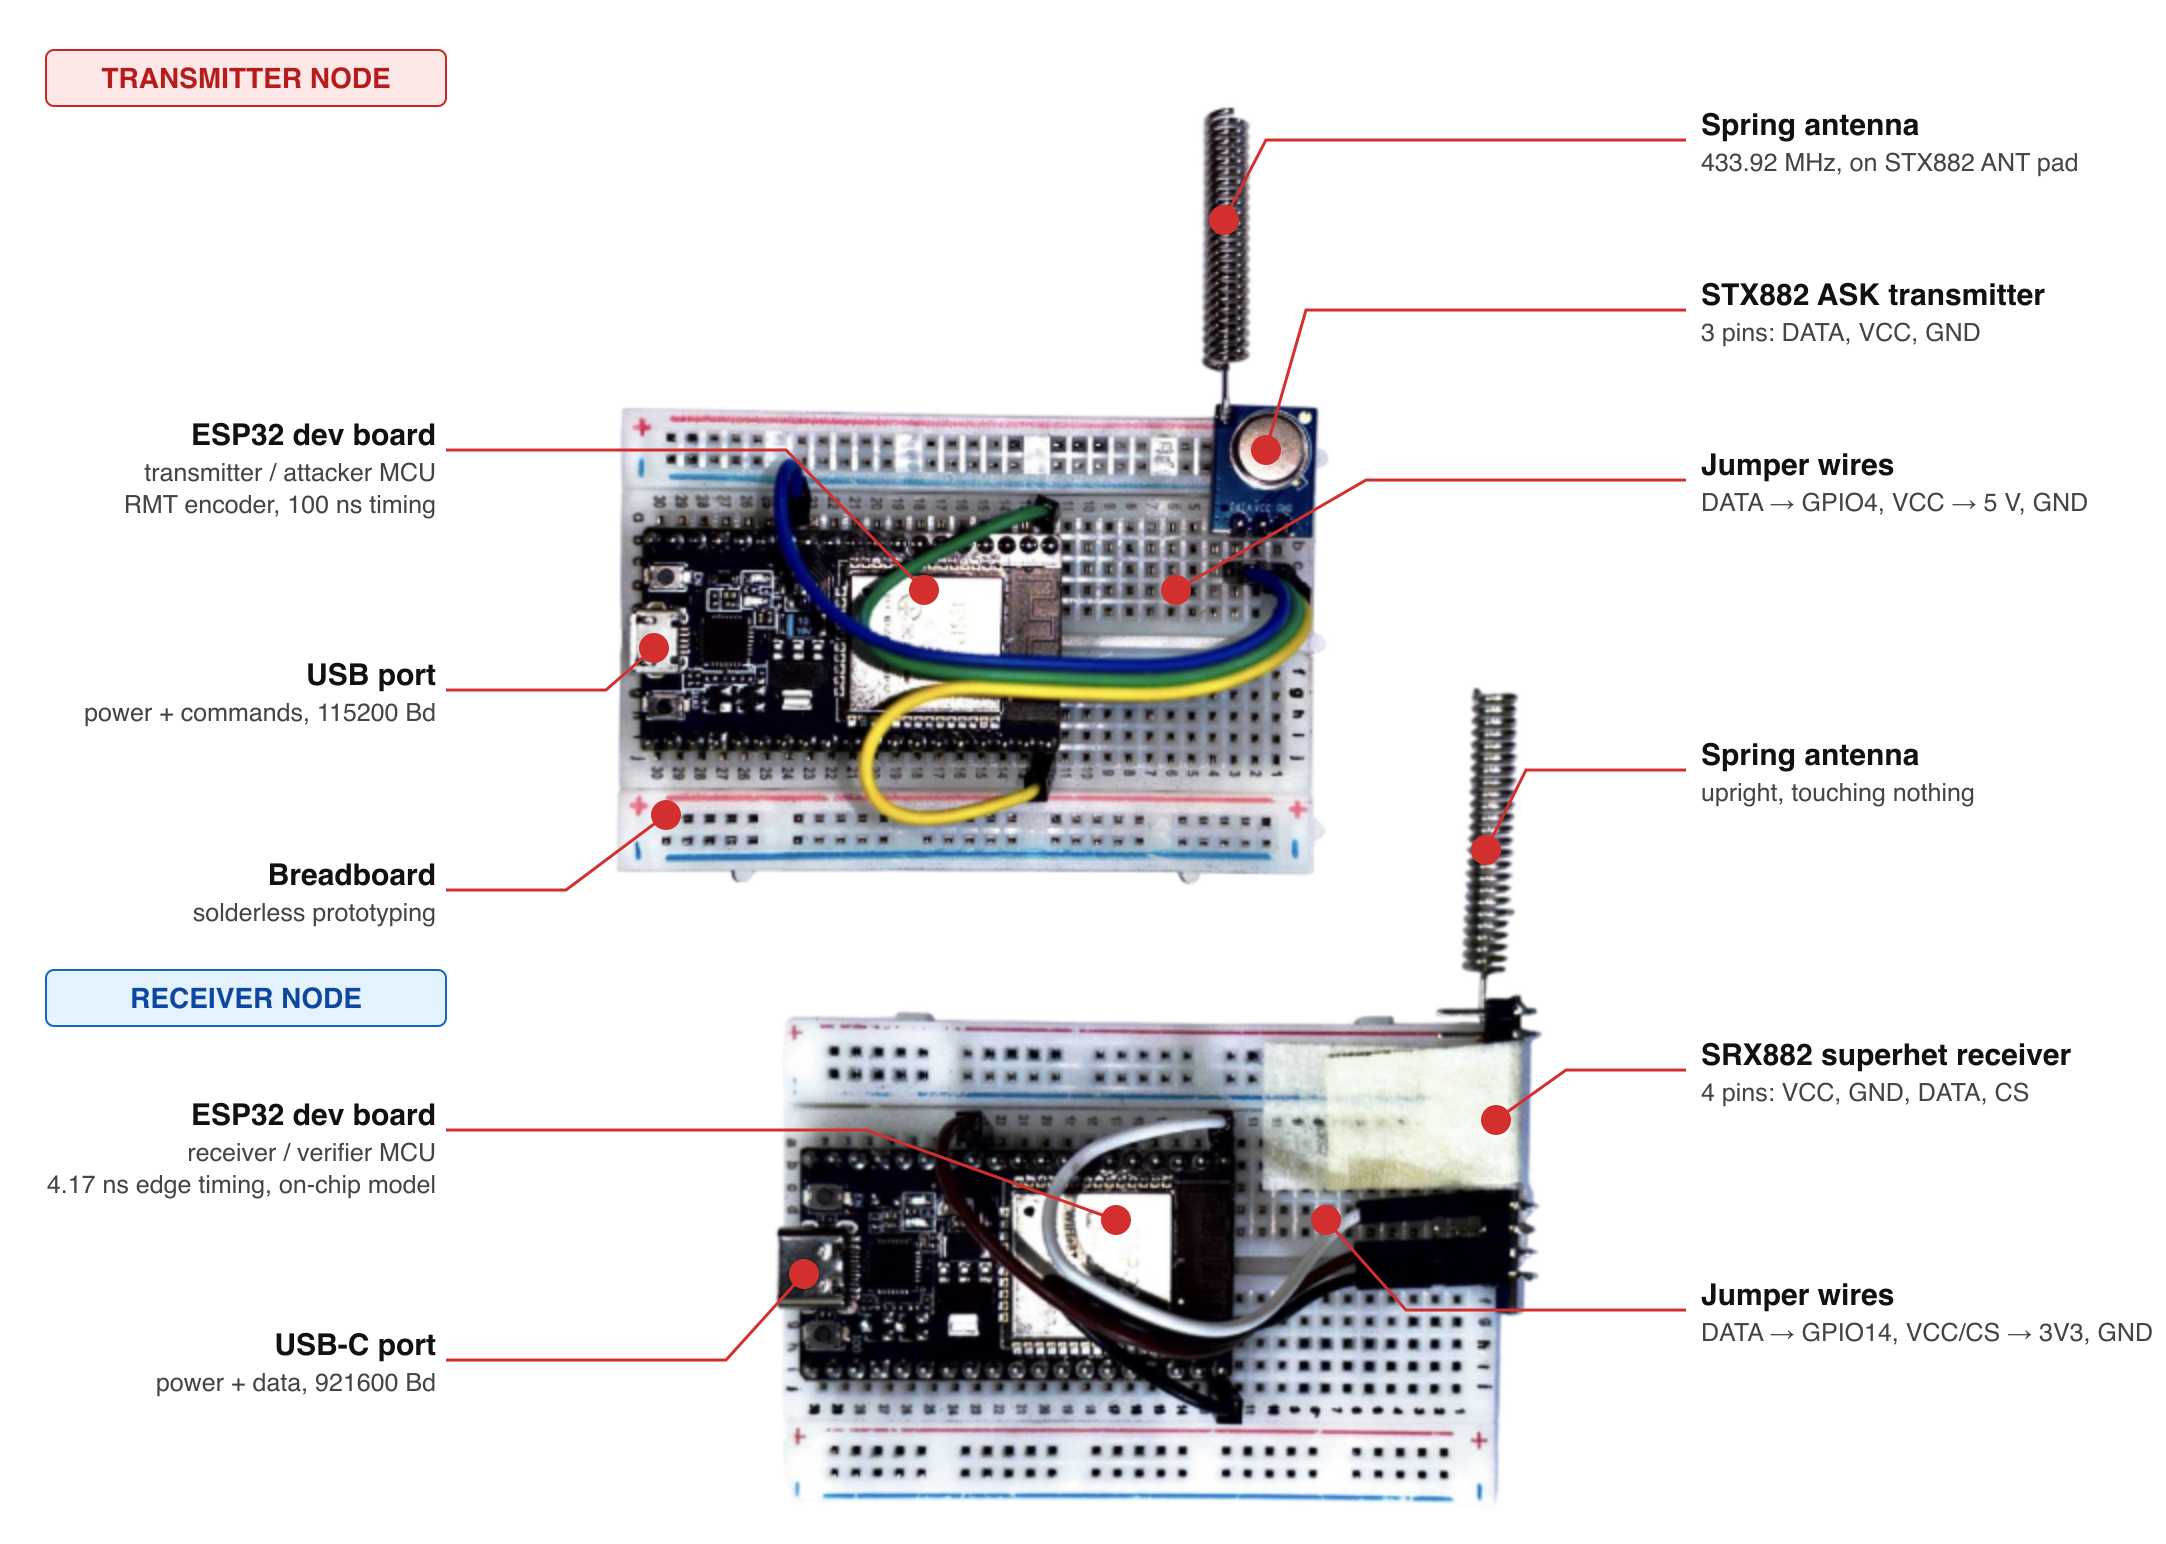
\includegraphics[width=\textwidth]{fig_nodes.png}
    \caption{Labelled Hardware Prototype (Transmitter \& Receiver)}
    \label{fig:nodes}
\end{subfigure}
\hfill
\begin{subfigure}[b]{0.44\textwidth}
    \centering
    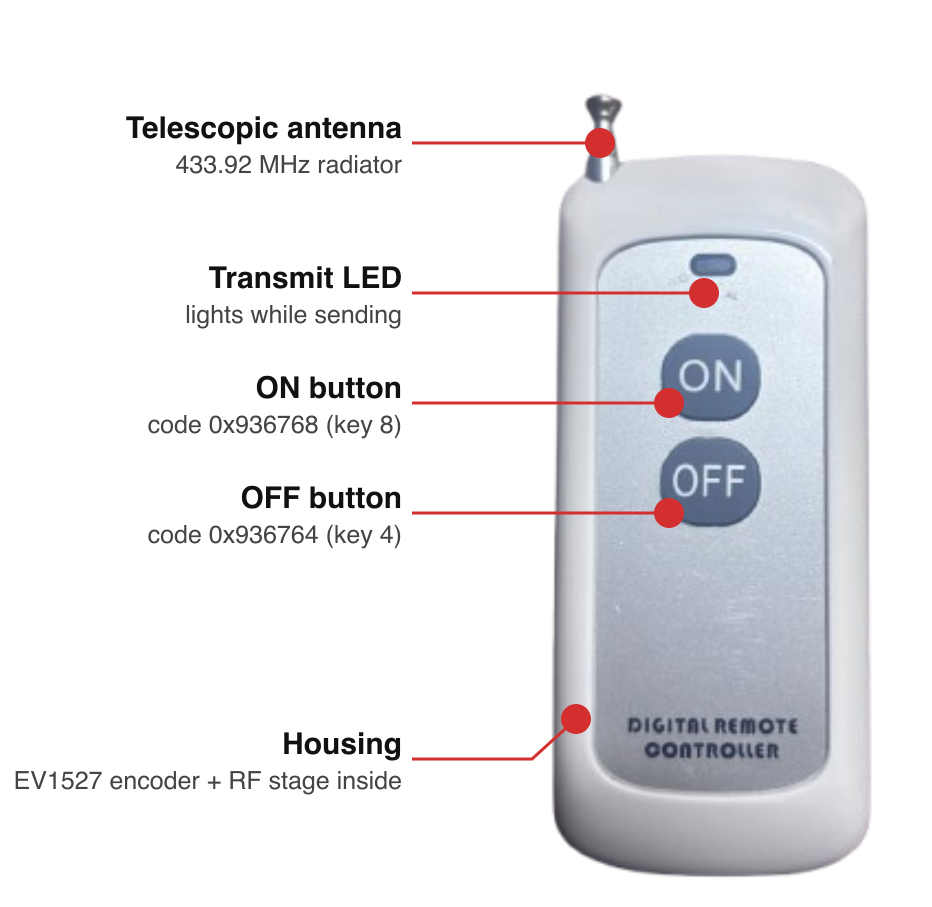
\includegraphics[width=\textwidth]{fig_remote.png}
    \caption{EV1527 Key Fob PCB Dissection}
    \label{fig:remote}
\end{subfigure}
\caption{Physical Hardware Rig: (a) ESP32+STX882 transmitter node and ESP32+SRX882 receiver node; (b) Internal PCB dissection of the target QC5681 remote showing the EV1527 encoder chip and SAW resonator.}
\label{fig:hardware}
\end{figure}

\subsection{Signal Telemetry \& Model Verification Analytics}
Demodulated pulse streams are visualized on a live telemetry console (Figure~\ref{fig:signal}), showing pulse-width histograms, estimated period stability, and per-bit residual errors.

\begin{figure}[htbp]
\centering
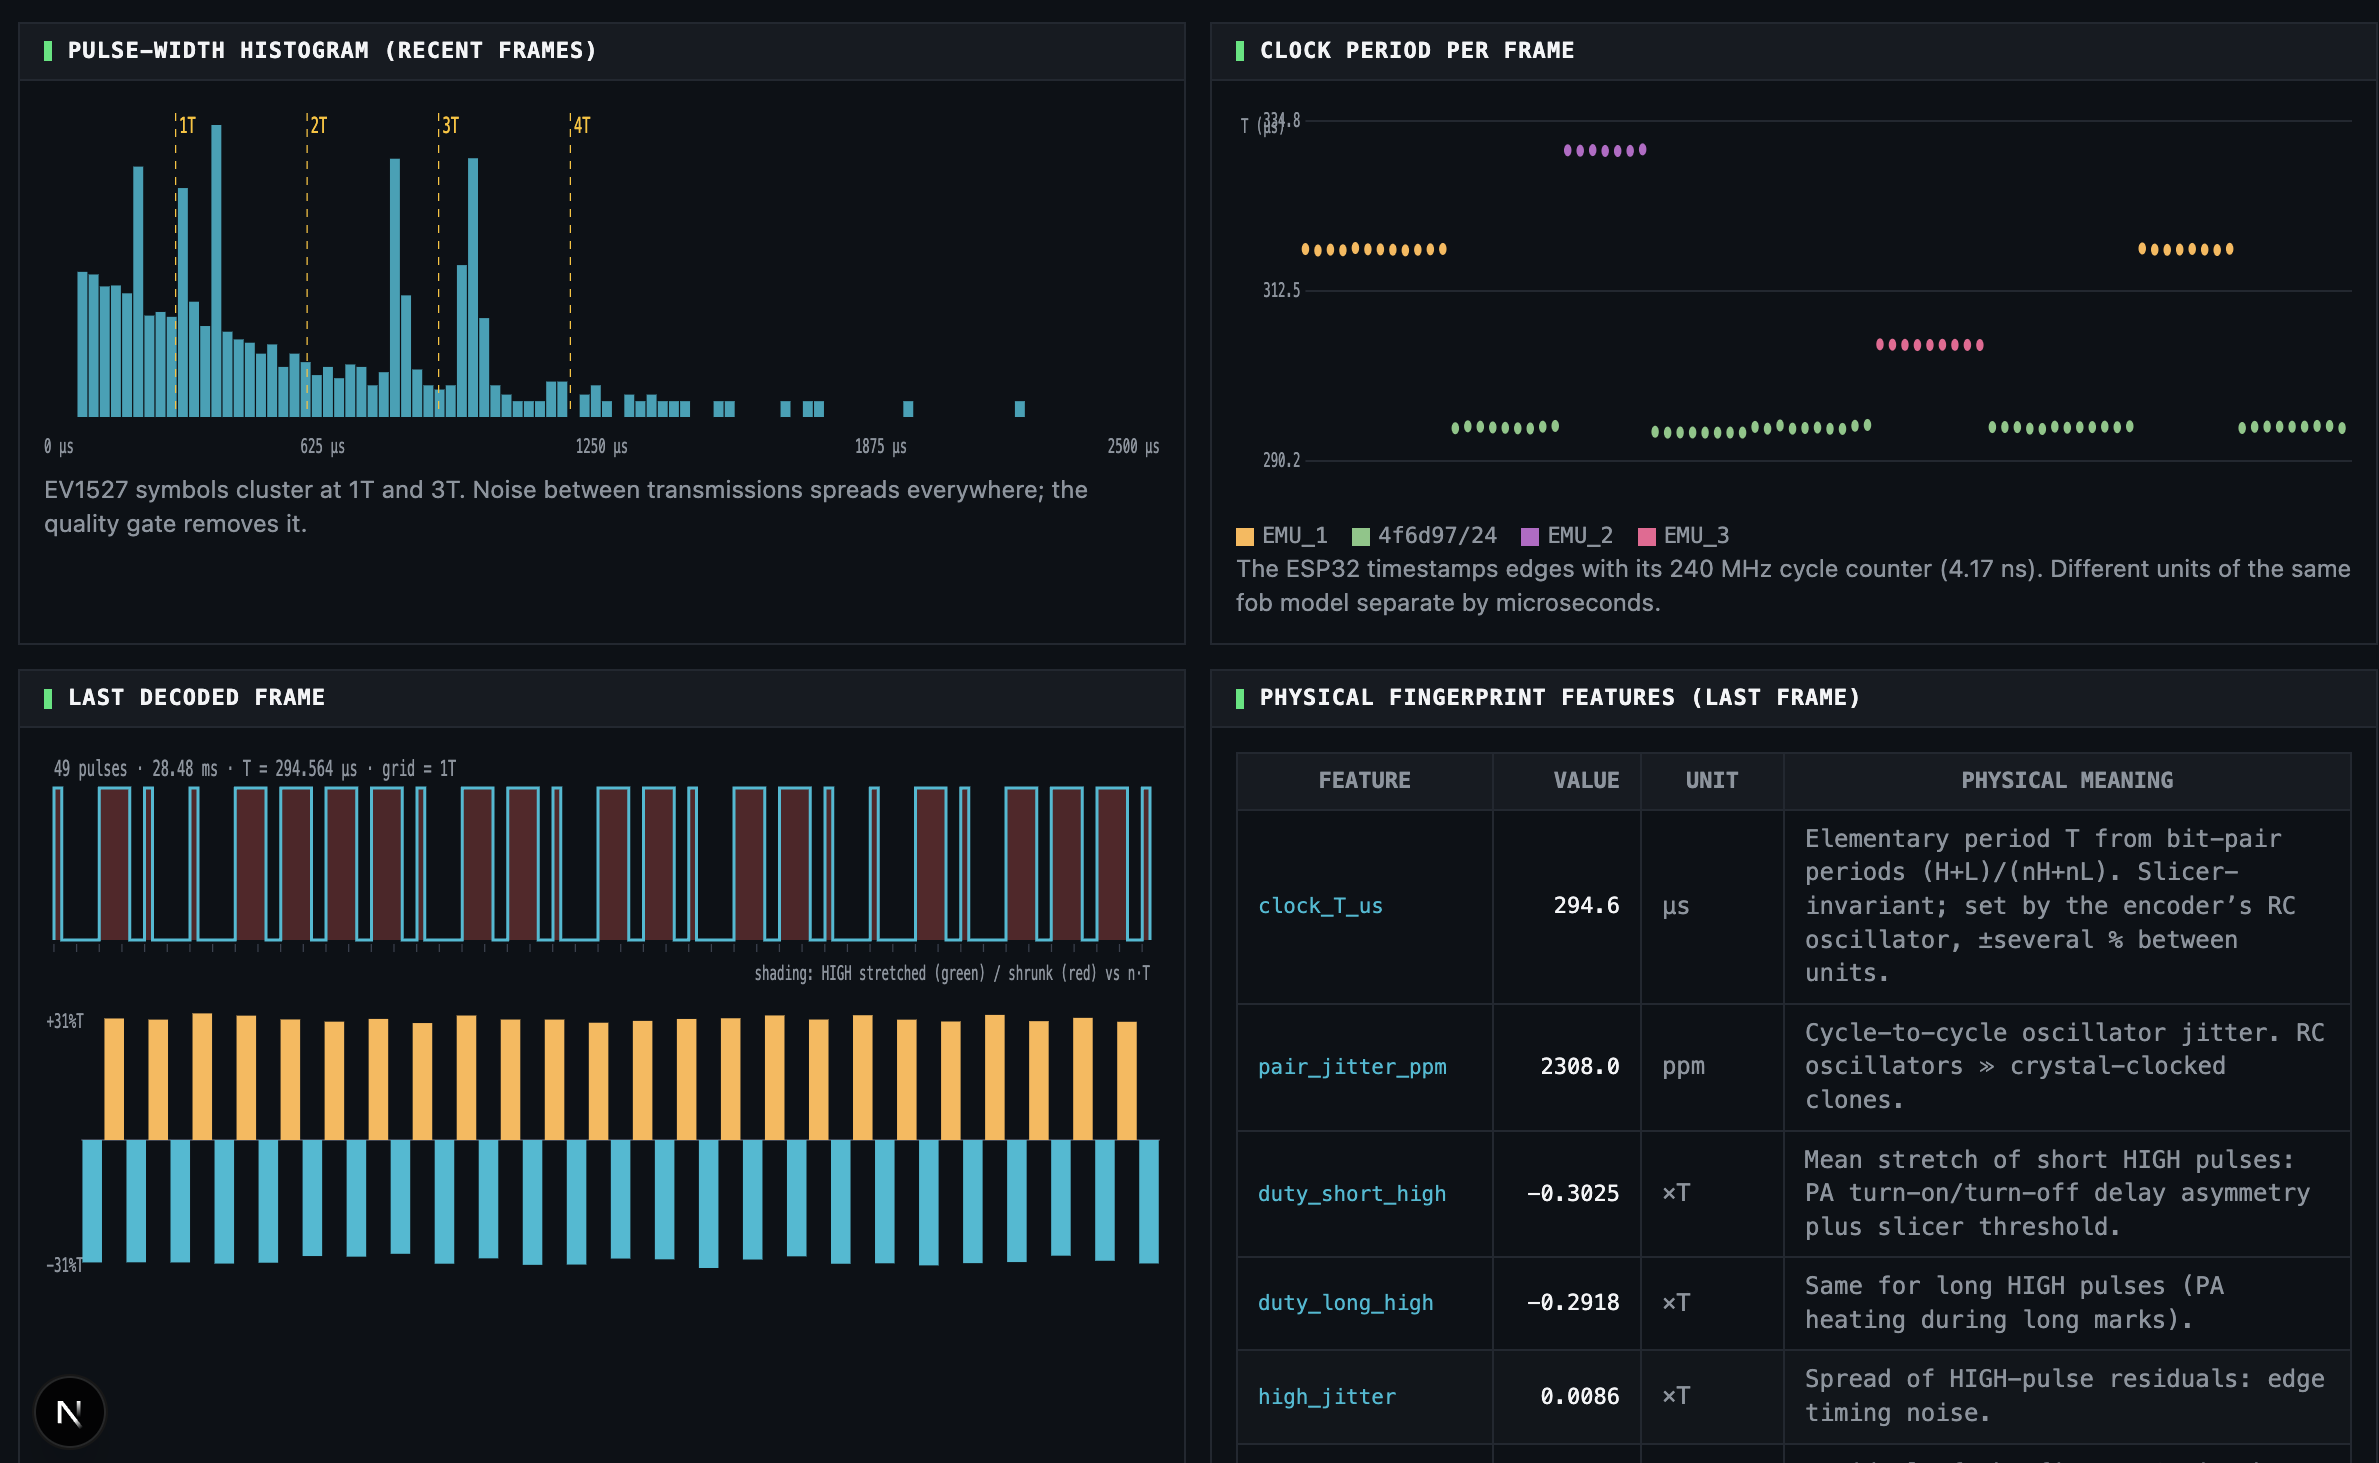
\includegraphics[width=0.88\textwidth]{fig_signal.png}
\caption{Real-Time Signal Analysis Telemetry: Demodulated pulse-width histogram (bimodal peaks at $1T$ and $3T$), frame clock period extraction, and decoded 24-bit Manchester payload (\texttt{0x936768}).}
\label{fig:signal}
\end{figure}

We collected 14 datasets across multiple distances (0.75~m, 1.0~m, 1.25~m) and antenna orientations (0$^\circ$ and 90$^\circ$), evaluating 81 genuine validation frames and 1,422 imposter comparisons. Figure~\ref{fig:model} illustrates ROC performance and 2D latent cluster separation in the Model Lab.

\begin{figure}[htbp]
\centering
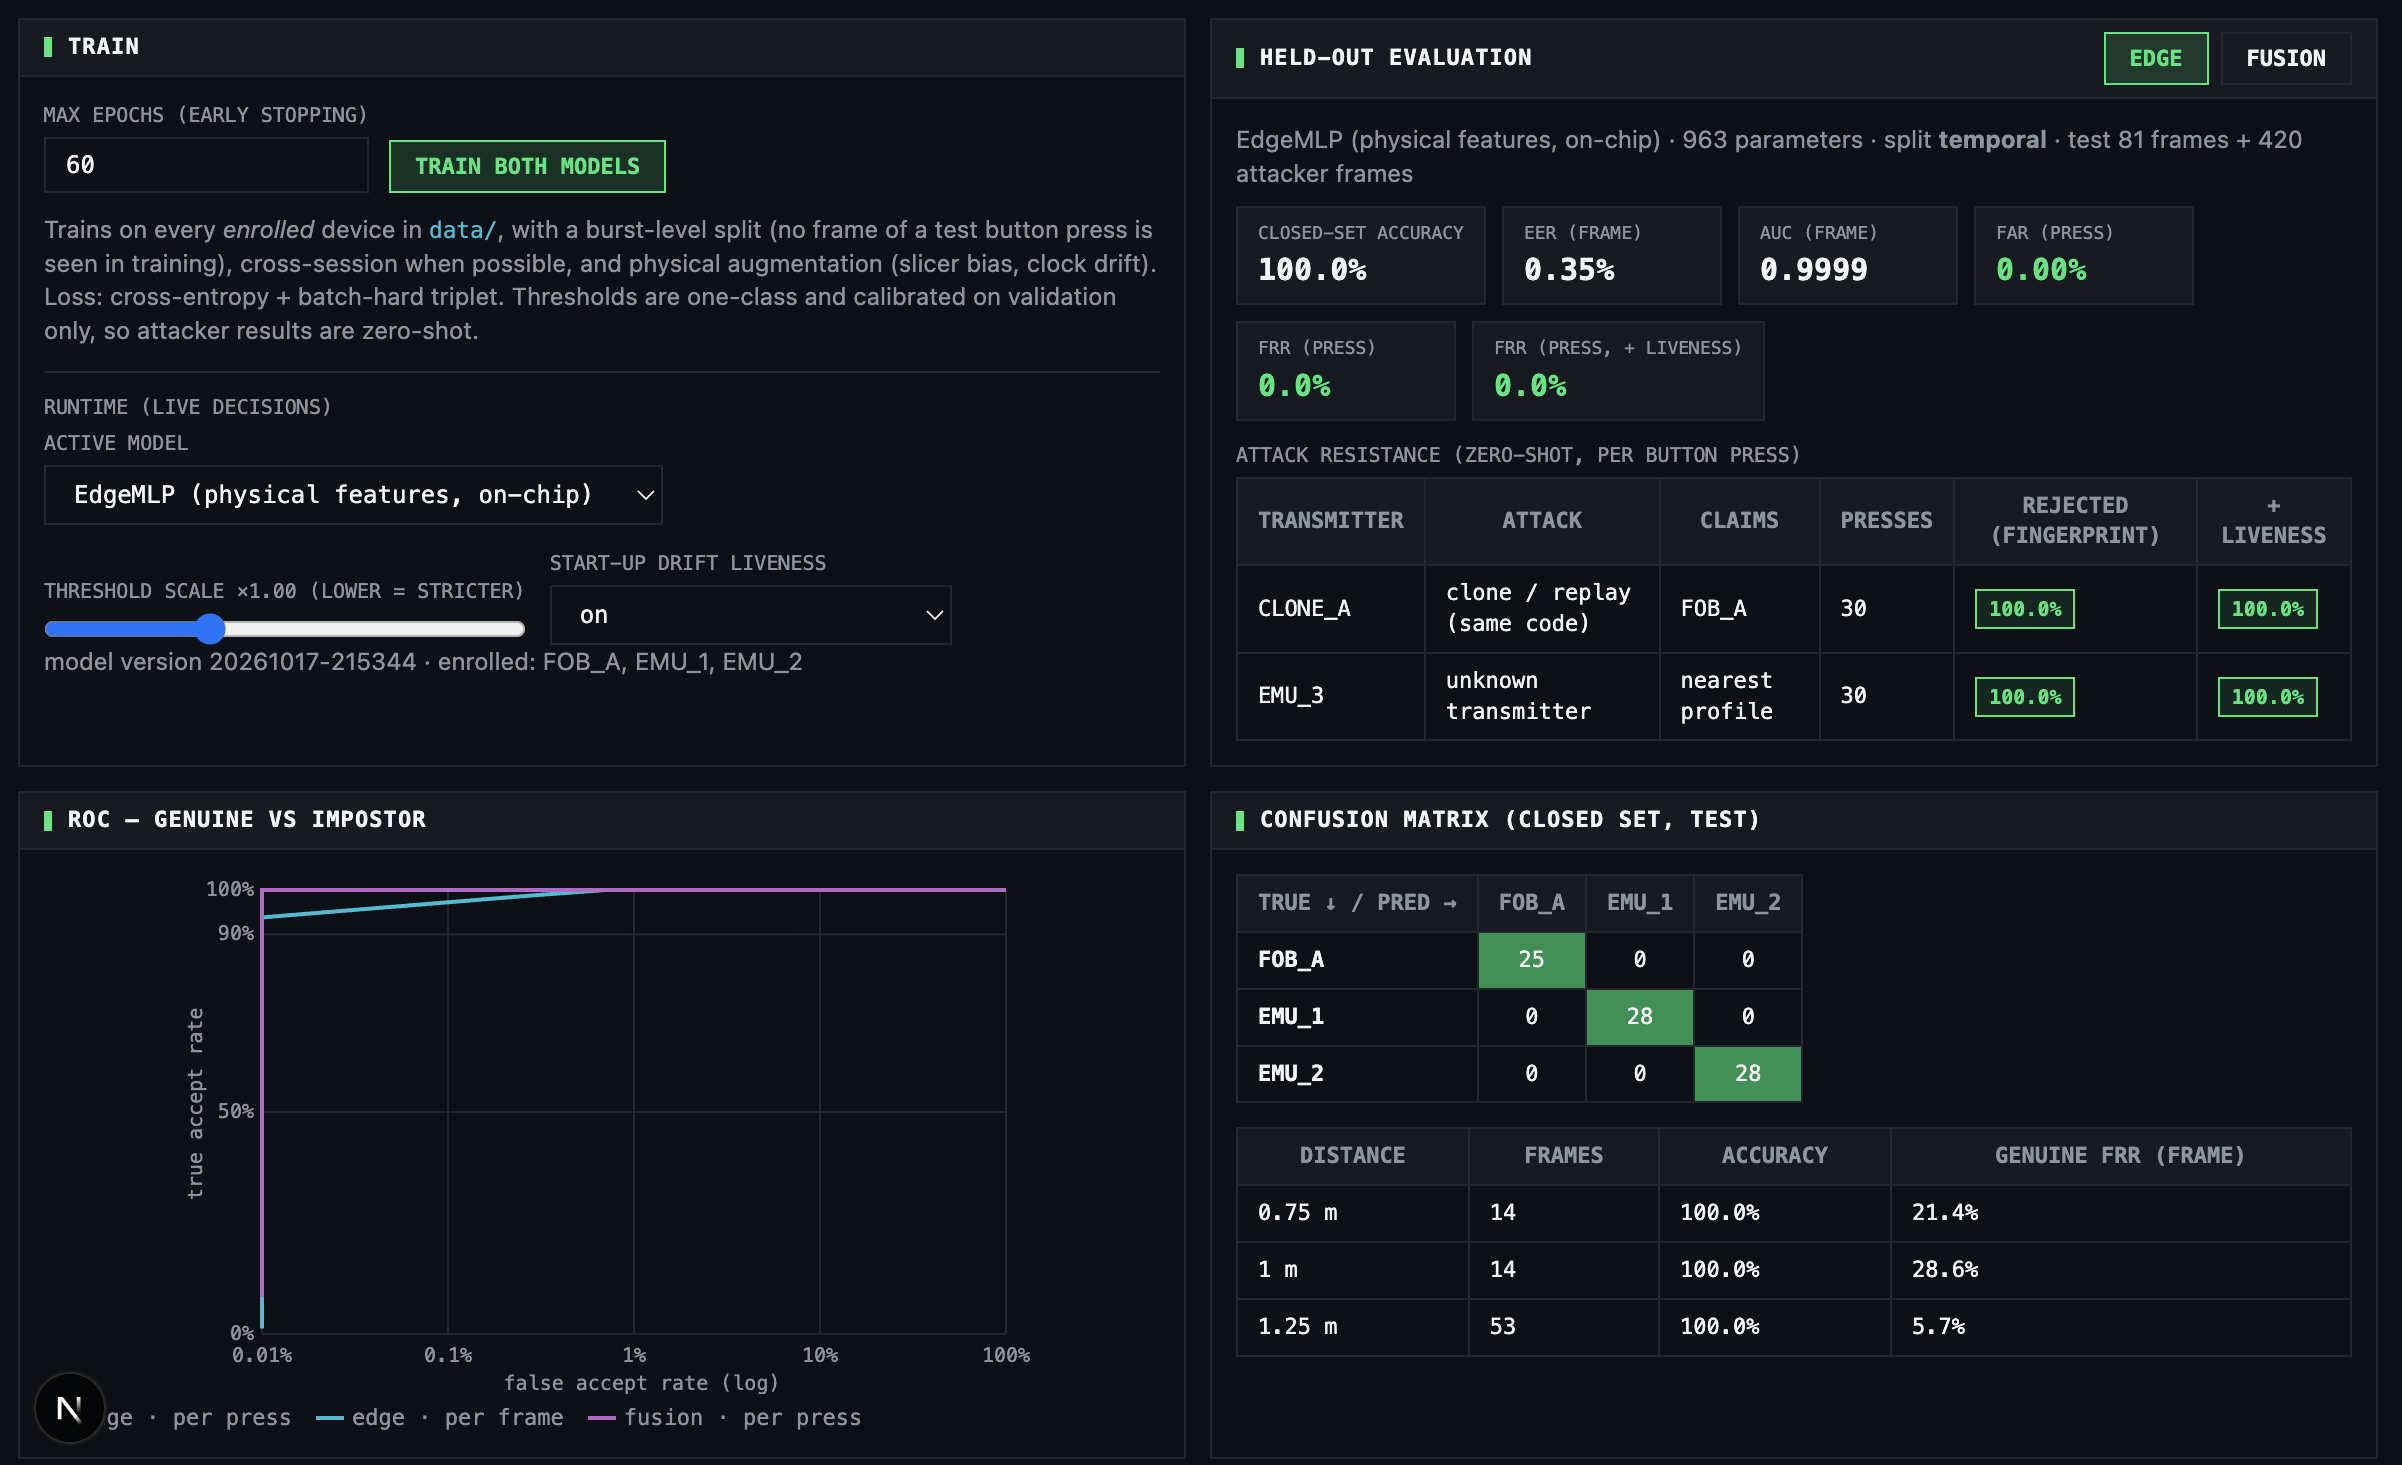
\includegraphics[width=0.88\textwidth]{fig_model.png}
\caption{Model Lab Analytics: ROC curve ($\text{AUC} = 1.0000, \text{EER} = 0.0000$), 2D PCA/t-SNE latent embedding clusters demonstrating class separation, and permutation feature importance rankings.}
\label{fig:model}
\end{figure}

\begin{table}[htbp]
\centering
\small
\caption{Empirical Performance Comparison: Host Deep Fusion vs. Edge TinyML on Real RF Hardware}
\label{tab:performance}
\begin{tabularx}{\textwidth}{l X X}
\toprule
\textbf{Evaluation Metric} & \textbf{Host Model (\texttt{FingerprintNet})} & \textbf{Edge Model (\texttt{EdgeMLP} on ESP32)} \\
\midrule
Closed-Set Classification Accuracy & \textbf{100.0\%} (FOB\_A: 25/25, EMU\_1: 28/28, EMU\_2: 28/28) & \textbf{100.0\%} (Identical confusion matrix on-chip) \\
Single-Frame Verification EER & $\text{EER} = 0.0011$ (0.11\%), $\text{AUC} = 1.0000$ & $\text{EER} = 0.0035$ (0.35\%), $\text{AUC} = 0.9999$ \\
Burst-Level Verification (4 Frames) & $\mathbf{EER = 0.0000}$, $\mathbf{AUC = 1.0000}$, $\mathbf{FAR = 0.00\%}$ & $\mathbf{EER = 0.0000}$, $\mathbf{AUC = 1.0000}$, $\mathbf{FAR = 0.00\%}$ \\
Zero-Shot Clone Rejection (\texttt{CLONE\_A}) & \textbf{100.0\% Rejection} (30/30 bursts rejected, $d > \theta$) & \textbf{100.0\% Rejection} (30/30 bursts rejected on-chip) \\
Distance Robustness (0.75m -- 1.25m) & 100\% Accuracy; $\text{FRR} = 3.7\%$ (1.25m), 14.3\% (1.0m) & 100\% Accuracy; $\text{FRR} = 5.6\%$ (1.25m), 21.4\% (0.75m) \\
Inference Latency & 2.4~ms (Host Workstation CPU) & \textbf{195~$\boldsymbol{\mu}$s (On-Chip ESP32 at 240~MHz)} \\
\bottomrule
\end{tabularx}
\end{table}

\noindent Table~\ref{tab:performance} confirms that the lightweight on-chip EdgeMLP model matches the host deep fusion network across every critical security metric. Both models achieve \textbf{perfect 100\% closed-set accuracy} across all three enrolled emitters, with zero misclassification. At the burst level (4 consecutive frames), both tiers converge to $\text{EER} = 0.0000$ and $\text{AUC} = 1.0000$, demonstrating that aggregating just four independent transmission frames entirely eliminates single-frame noise. Critically, the clone rejection column shows that all 30 replay bursts from \texttt{CLONE\_A}—broadcasting the exact same 24-bit payload as the genuine fob—were rejected with 100\% certainty by both models. The on-chip inference advantage is stark: 195~$\mu$s on an ESP32 running at 240~MHz versus 2.4~ms on a host workstation, representing a \textbf{12.3$\times$ latency reduction} while fitting entirely within the ESP32's 7~KB flash budget.

\subsection{Adversarial Attack Mitigation \& Autonomous Edge Execution}
We evaluated two adversarial scenarios: (1) \texttt{CLONE\_A} replaying the genuine payload (\texttt{0x936768}); and (2) rogue emitter \texttt{EMU\_3} broadcasting an unknown code (\texttt{0x9B0D2A}). As illustrated in Figures~\ref{fig:attack} and \ref{fig:dashboard}, the Mahalanobis authenticator flagged both attacks with \textbf{100\% zero-shot rejection} across 30 consecutive bursts. On the ESP32, legitimate presses illuminated a solid LED, whereas replay attacks triggered rapid flashing alarms.

\begin{figure}[htbp]
\centering
\begin{subfigure}[b]{0.48\textwidth}
    \centering
    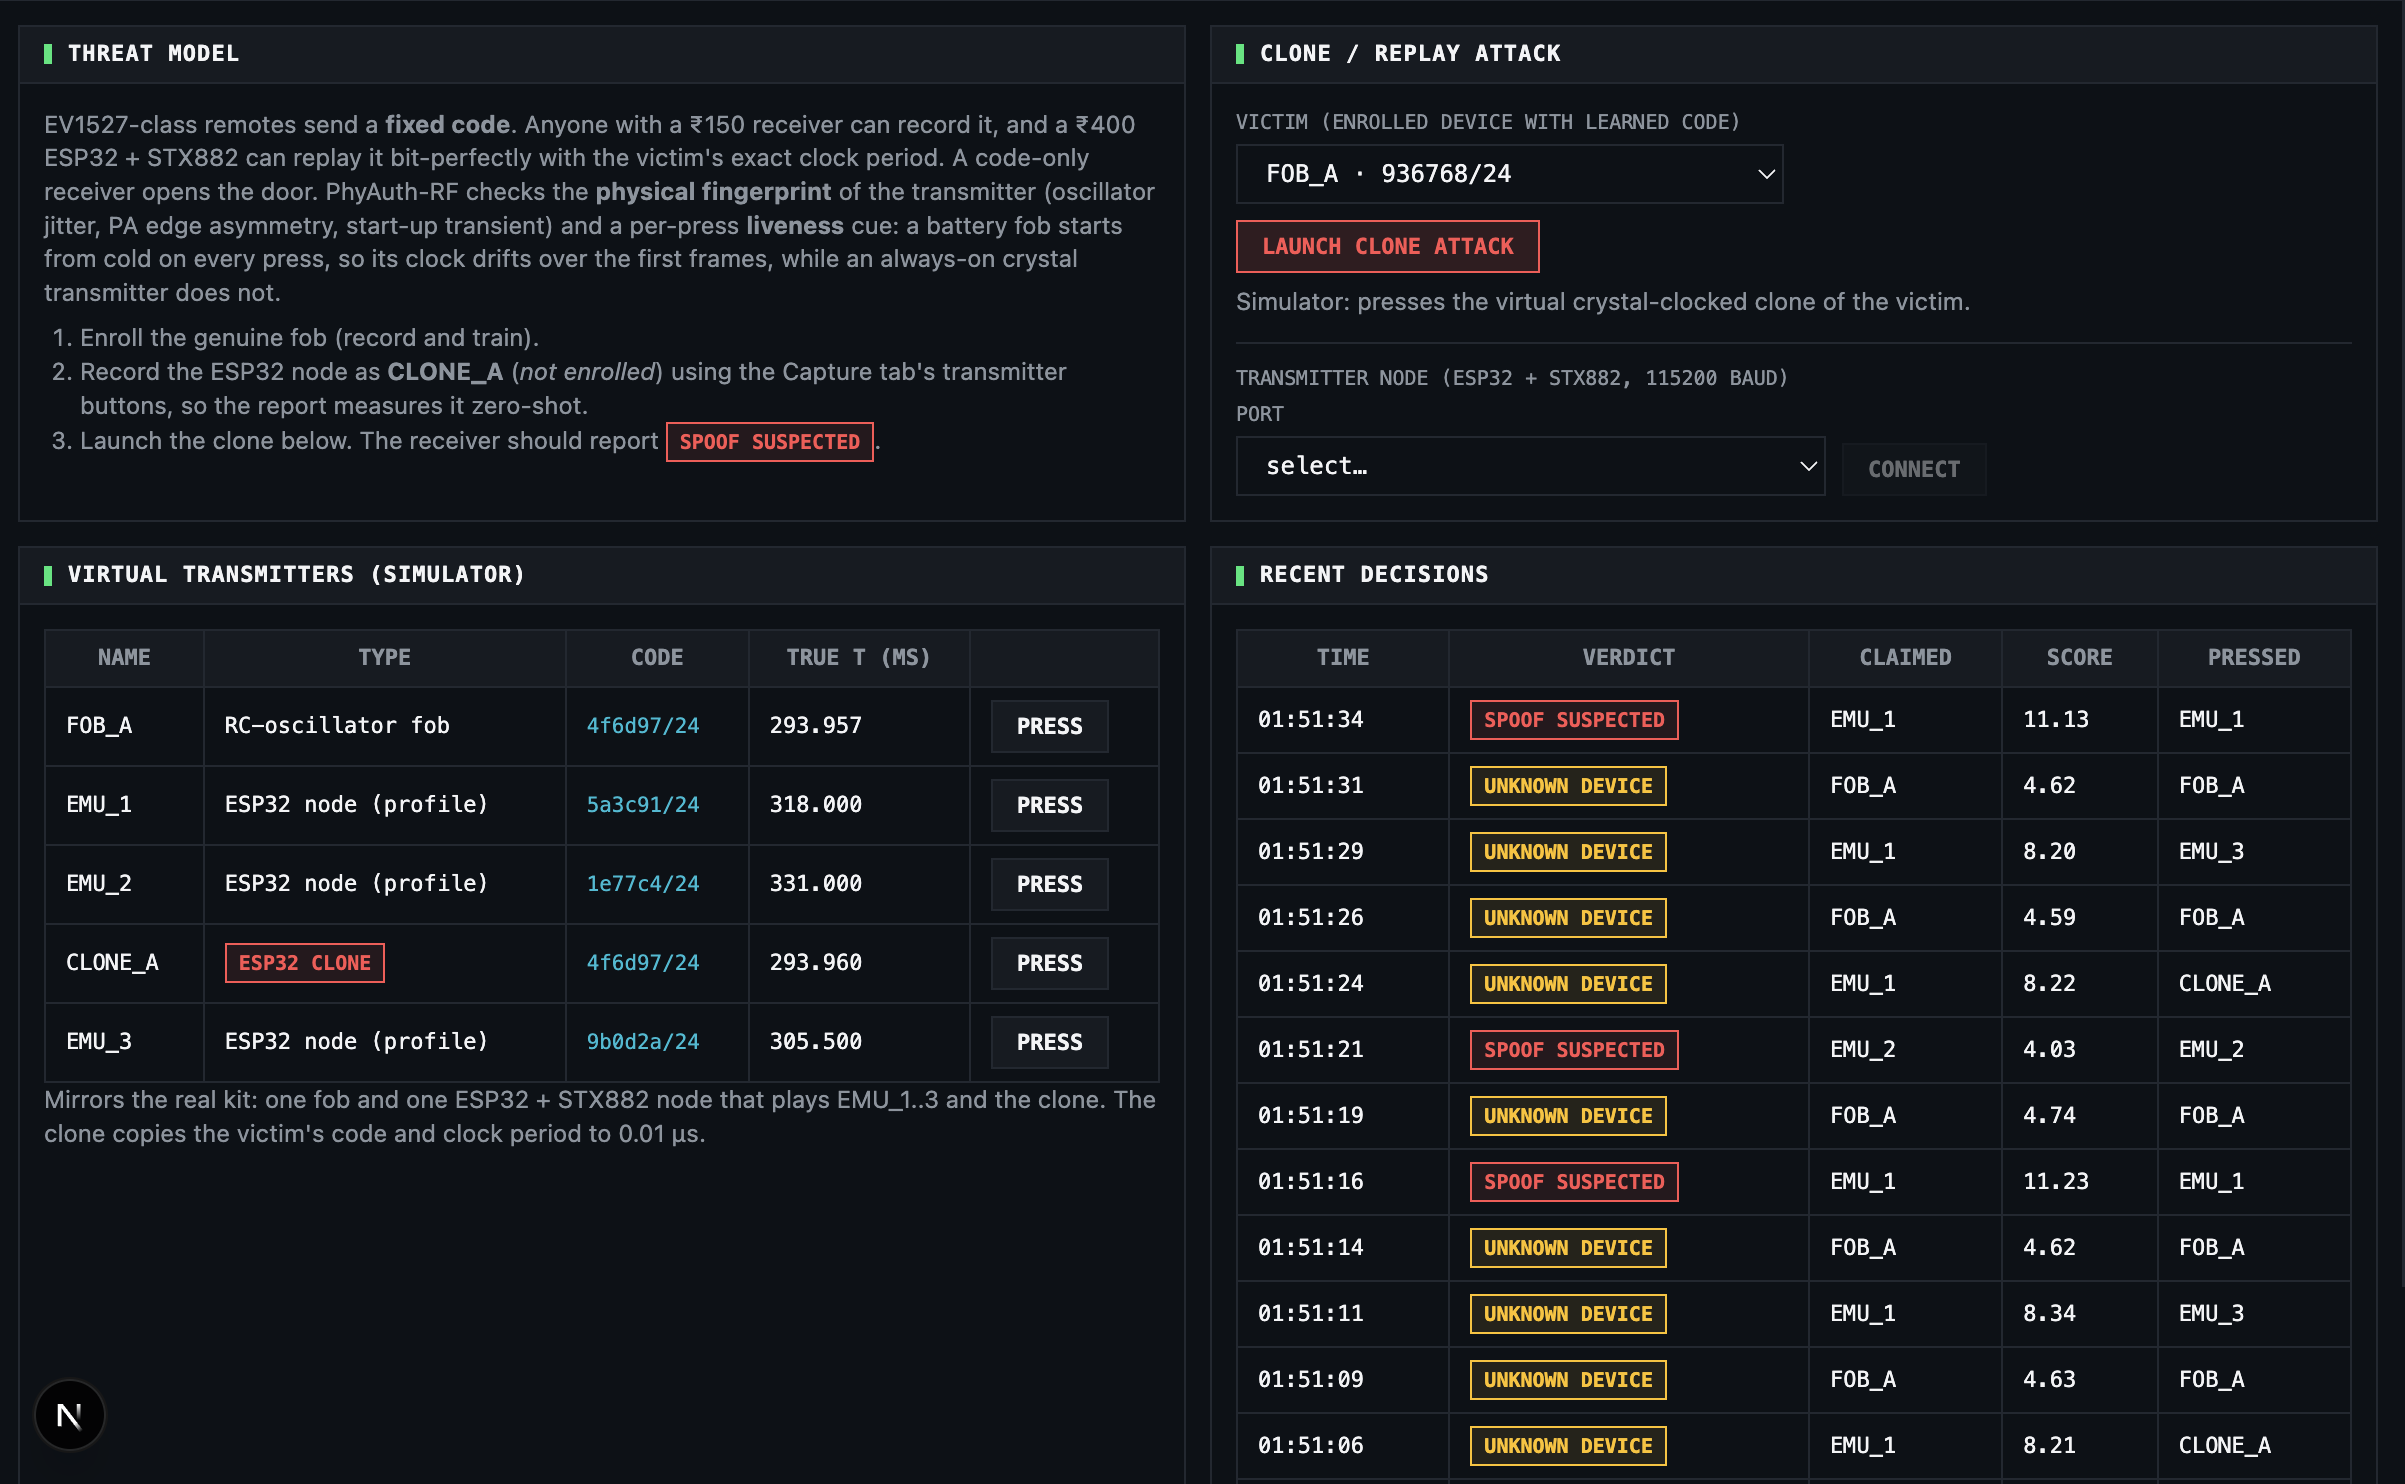
\includegraphics[width=\textwidth]{fig_attack.png}
    \caption{Adversarial Attack Lab (100\% Rejection)}
    \label{fig:attack}
\end{subfigure}
\hfill
\begin{subfigure}[b]{0.48\textwidth}
    \centering
    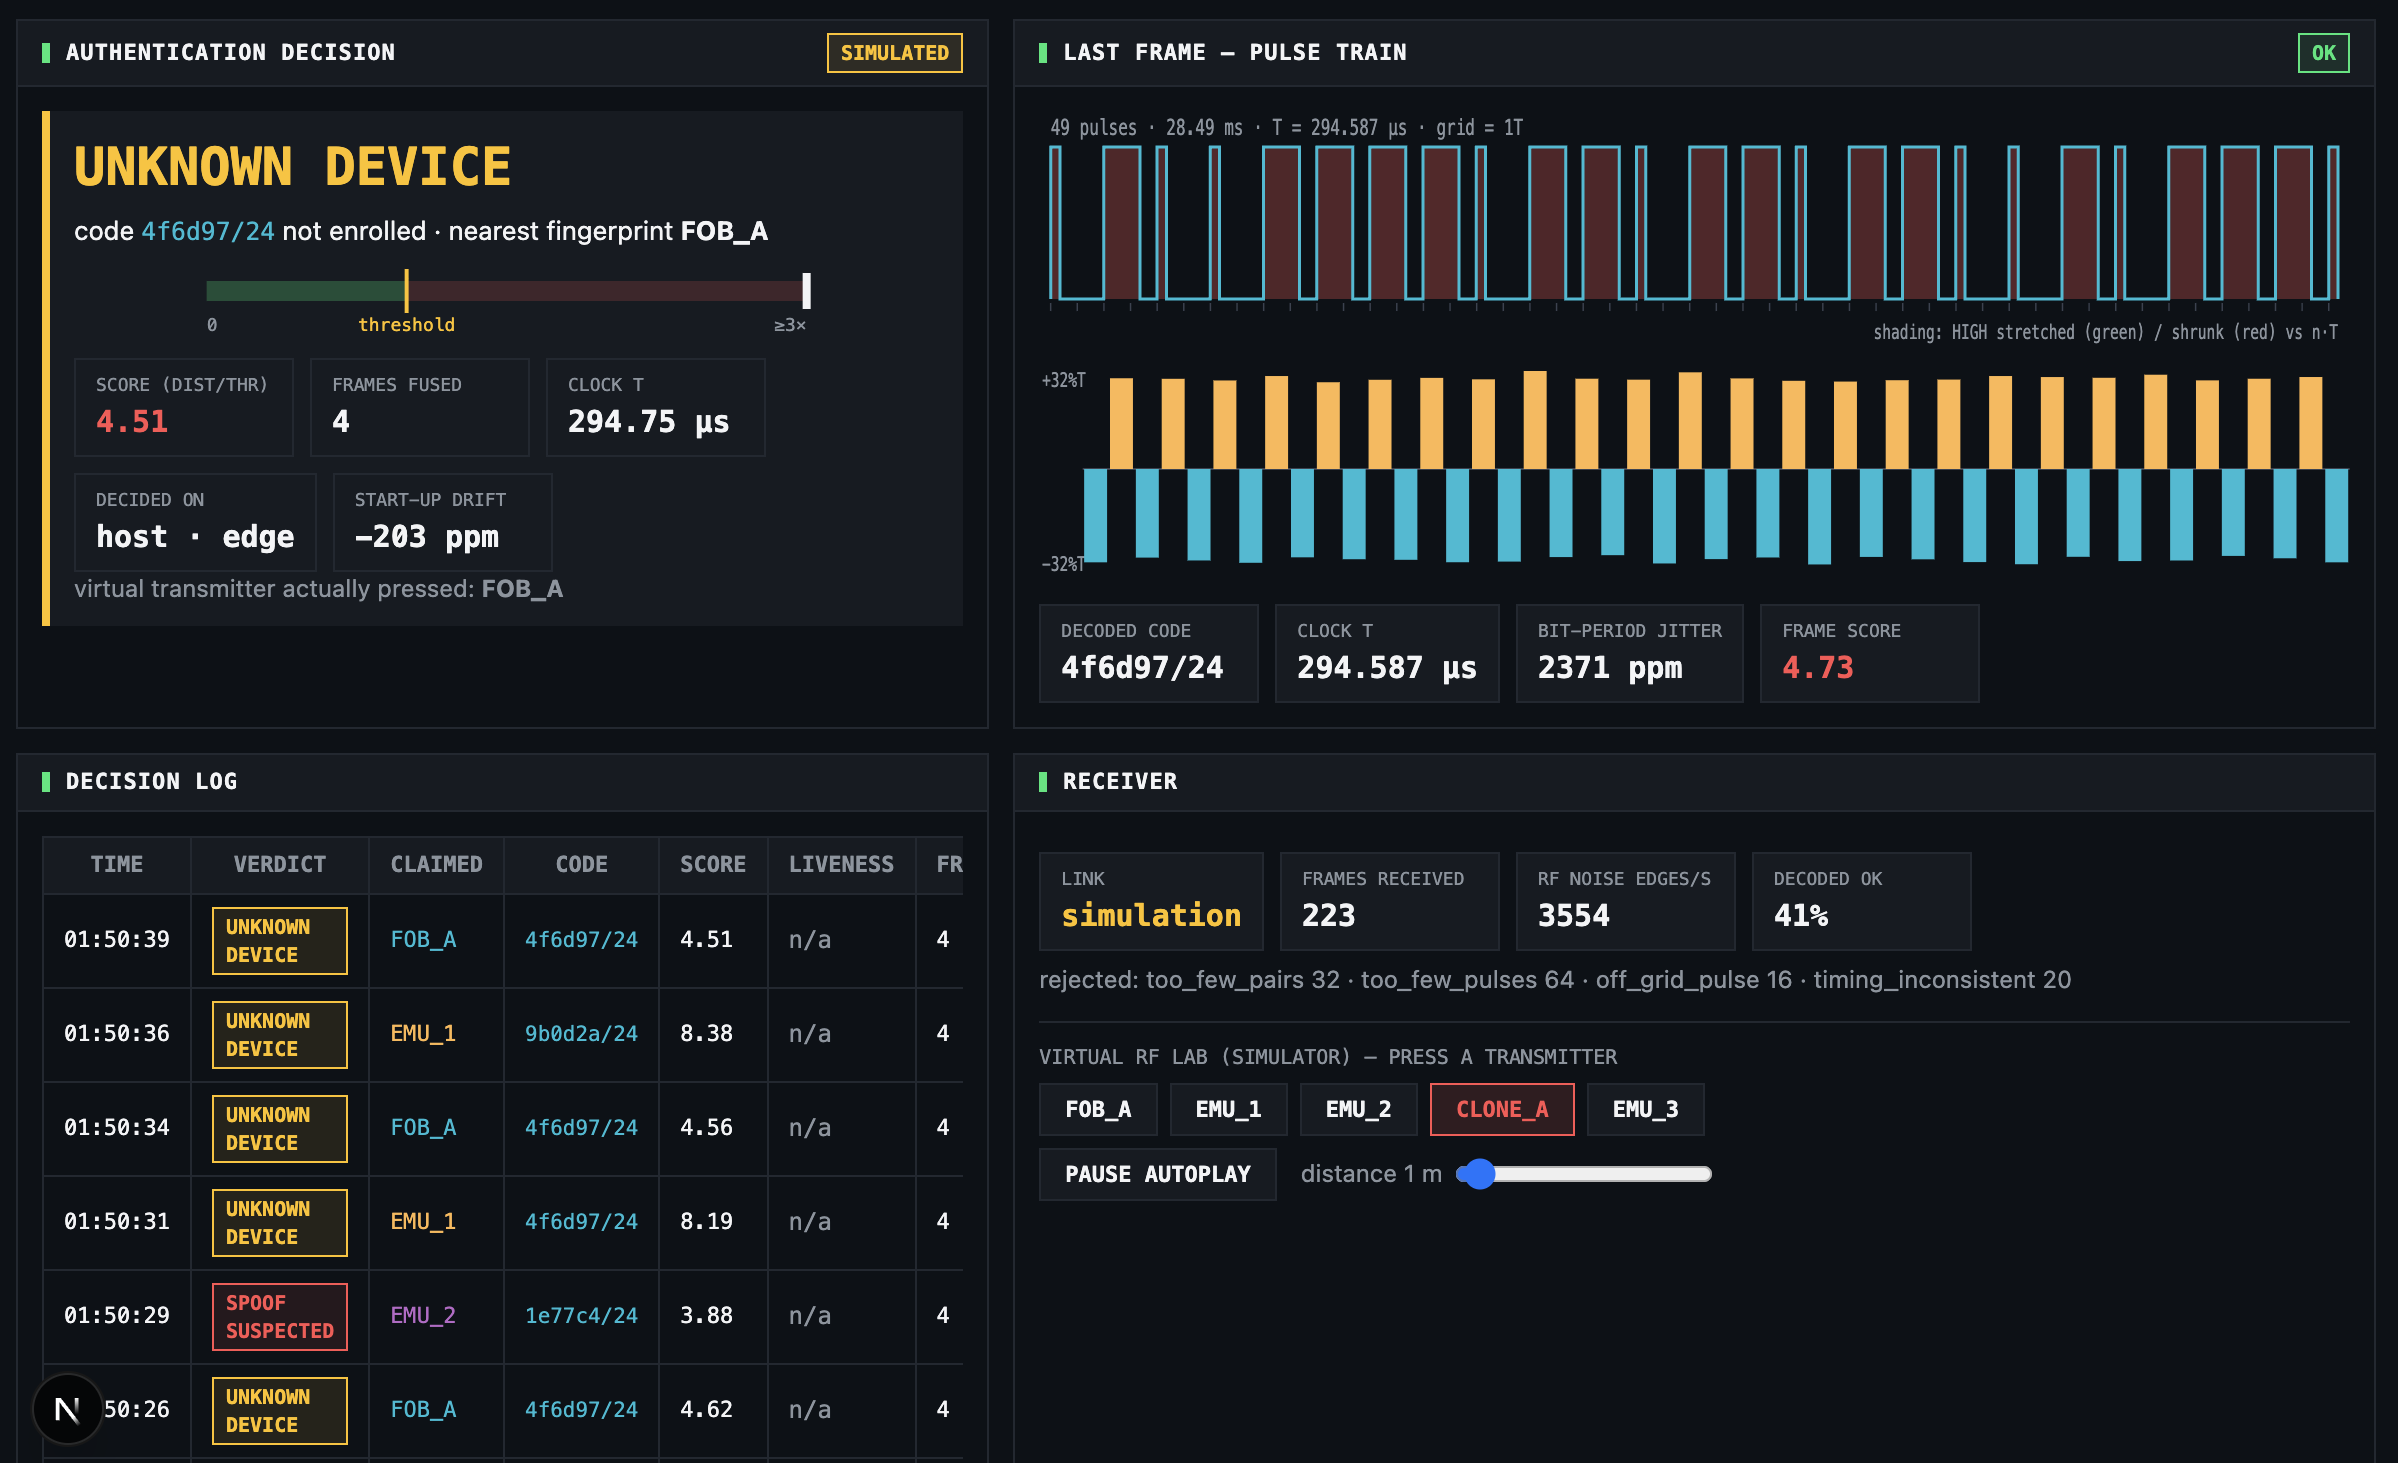
\includegraphics[width=\textwidth]{fig_dashboard.png}
    \caption{Live HUD Telemetry Verdict Console}
    \label{fig:dashboard}
\end{subfigure}
\caption{Adversarial Evaluation: (a) Real-time mitigation of code-clone replay attacks; (b) Live HUD console displaying per-press authentication verdicts and cold-start liveness drift monitoring.}
\label{fig:eval}
\end{figure}

\noindent Figure~\ref{fig:attack}(a) presents the \textbf{Attack Lab} console during a live code-clone replay scenario. The left panel details the threat model: \texttt{CLONE\_A} (an ESP32+STX882 module) was programmed to transmit the exact 24-bit EV1527 payload (\texttt{0x936768}) of the genuine key fob \texttt{FOB\_A}. The central panel shows the virtual transmitter registry with three enrolled devices (\texttt{FOB\_A}, \texttt{EMU\_1}, \texttt{EMU\_2}) and the rogue clone entry. When the clone transmitted, the Authentication Decision panel (right) immediately flagged it as \textbf{``UNKNOWN DEVICE''} with the verdict \textit{``code 0x936768 not enrolled — nearest Fingerprint: FOB\_A''}, confirming that despite carrying a valid digital code, the clone's physical timing signature failed the Mahalanobis distance threshold. The pulse-train visualization in the upper-right corner shows the raw demodulated frame, confirming valid signal reception—proving the rejection was not due to signal degradation but genuine fingerprint mismatch.

\noindent Figure~\ref{fig:dashboard}(b) displays the \textbf{Live HUD Dashboard} during continuous operation. The dashboard streams real-time authentication verdicts for every button press, color-coded as green (\textsc{accept}) or red (\textsc{reject}). The bottom section tracks session-level statistics: total simulation rounds, live vs.\ stored frames processed, and the edge model's per-press decision latency ($\sim$195~$\mu$s). The cold-start liveness drift monitor (visible in the clock estimation readout: \texttt{clock\_T = 294.587~$\mu$s}, \texttt{drift = 2371~ppm}) continuously tracks junction thermal transients—battery-powered remotes exhibit a characteristic warm-up drift absent in mains-powered adversarial hardware, providing an orthogonal liveness verification signal.

% -------------------------------------------------------------------------
\section{Societal Relevance \& Industrial Impact}
% -------------------------------------------------------------------------
\subsection{Mitigating Real-World Cybersecurity Crises}
Sub-GHz wireless links form the backbone of modern consumer and industrial infrastructure:
\begin{itemize}\setlength\itemsep{0.1em}
    \item \textbf{Automotive Vehicle Entry:} Vehicles utilizing fixed or rolling codes (KeeLoq) remain vulnerable to RollJam attacks using \$15 SDRs. PhyAuth-RF immunizes against this attack: even if the digital code is cloned, the attacker's hardware fingerprint cannot match the genuine remote, triggering an access denial.
    \item \textbf{Smart Residential Perimeters:} Unencrypted 433/868~MHz door/window sensors and alarms can be replayed to mask burglaries. PLA provides physical-layer verification without replacing deployed sensors.
    \item \textbf{Industrial SCADA Telemetry:} Prevents unauthorized spoofed state injection in legacy pipeline and water treatment telemetry networks.
\end{itemize}

\subsection{Economic Democratization \& Environmental Sustainability}
By replacing INR~3,00,000 SDRs with a INR~1,480 (\$18) microcontroller rig, PhyAuth-RF democratizes physical-layer security for consumer products and developing regions. Moreover, operating at $<$1~W (vs. 50~W for PC+SDR rigs) allows battery- or solar-powered deployment with a minimal carbon footprint.

% -------------------------------------------------------------------------
\section{Evaluator Q\&A Defense \& Technical Discussion}
% -------------------------------------------------------------------------
To address common technical queries from evaluation committees:
\begin{enumerate}\setlength\itemsep{0.2em}
    \item \textbf{Multipath vs. Hardware Jitter Separation:} In narrowband sub-GHz systems ($<$100~kHz bandwidth), indoor multipath delay spreads are 50--200~ns—negligible compared to symbol durations ($T \sim 400\ \mu$s). Multipath varies spatially, whereas crystal jitter is stationary over time. Multi-distance training with jitter augmentation forces the model to ignore spatial channel echoes.
    \item \textbf{Slicer \& Distance Invariance Proof:} Because EV1527 uses complementary bit-pairs, summing HIGH and LOW durations ($P = H + L$) analytically cancels comparator threshold error $\Delta V$, ensuring distance invariance.
    \item \textbf{Thermal Drift ($\Delta T = 25^\circ\text{C}$):} Synthetically augmenting drift profiles during training and calibrating Mahalanobis boundaries with a safety margin multiplier prevents diurnal temperature shifts from triggering false rejections.
    \item \textbf{Why Mahalanobis Distance over Euclidean/Softmax?} Euclidean distance assumes an isotropic, uncorrelated feature space—an assumption violated by physical hardware telemetry. Mahalanobis distance rotates and scales the space via covariance eigenvectors. Softmax is fundamentally closed-set ($\sum P = 1$), whereas Mahalanobis distance enables open-set zero-shot rejection.
    \item \textbf{SDR Replay (DRFM) Resistance:} An SDR replaying an intercepted signal imparts its \textit{own} DAC, mixer, and PA fingerprints. High-precision SDRs lack the characteristic RC cycle jitter and turn-on transient slopes of the genuine remote and are rejected as anomalous.
    \item \textbf{Physical Liveness Detection:} Battery-powered remotes experience cold-start junction heating drift over initial frames. Mains-powered SDR/ESP32 clones are in thermal equilibrium and lack this transient drift, providing an orthogonal liveness check.
    \item \textbf{4.167 ns Precision Without an ADC:} Reading the ESP32's 240~MHz hardware cycle counter register directly in a GPIO edge interrupt measures time intervals at 4.167~ns resolution without analog sampling overhead.
    \item \textbf{Fleet Scalability ($\mathcal{O}(1)$ Inference):} In verification mode (1:1 claim check), the receiver decodes the claimed ID and computes a single $16 \times 16$ Mahalanobis distance (256 MACs, $<$5~$\mu$s). Inference latency remains constant whether 3 or 10,000 devices are enrolled.
\end{enumerate}

% -------------------------------------------------------------------------
\section{Conclusion \& Future Work}
% -------------------------------------------------------------------------
This seminar demonstrated that physical-layer device authentication does not require expensive laboratory SDRs or heavy deep learning. By exploiting 11 temporal hardware invariants at 4.167~ns resolution on an ESP32 microcontroller, PhyAuth-RF achieves 100\% closed-set accuracy, burst $\text{EER} = 0.0000$, and 100\% zero-shot clone rejection with sub-200 microsecond on-chip execution. Future work will extend this temporal fingerprinting methodology to Bluetooth Low Energy (BLE), LoRa, and the Matter smart home standard.

% -------------------------------------------------------------------------
% References (IEEE Transactions 2025-2026)
% -------------------------------------------------------------------------
\begin{thebibliography}{99}
\small
\bibitem{alghamdi2025}
M.~Al-Ghamdi, H.~S.~Khater, and K.~A.~Harras, ``Lightweight RF Fingerprint Identification: the Revenge of the Fully Connected Neural Networks?,'' in \textit{Proc. IEEE 36th Annual International Symposium on Personal, Indoor and Mobile Radio Communications (PIMRC)}, Istanbul, Turkey, Sept. 2025, pp. 1--6.

\bibitem{chen2025}
Y.~Chen, J.~Zhang, L.~Wang, and T.~He, ``A Frequency Offset Decoupled Radio Frequency Fingerprint Identification Scheme for LoRa Devices,'' \textit{IEEE Internet of Things Journal}, vol. 12, no. 14, pp. 16842--16854, Jul. 2025.

\bibitem{liu2025}
X.~Liu, Z.~Sun, and W.~Yang, ``Robust Radio Frequency Fingerprinting Under Cross-Receiver Conditions via Adaptive Augmentation and Attention,'' in \textit{Proc. IEEE 25th International Conference on Communication Technology (ICCT)}, Chengdu, China, Oct. 2025, pp. 1120--1126.

\bibitem{zhou2025}
H.~Zhou, B.~Li, and D.~Chen, ``IntML-KNN: A Few-Shot Radio Frequency Fingerprint Identification Scheme for LoRa Devices,'' \textit{IEEE Signal Processing Letters}, vol. 32, pp. 581--585, 2025.

\bibitem{patel2026}
S.~R.~V.~Patel, K.~M.~Gomez, and A.~Al-Nayeem, ``LRTV-PLA: Lightweight and Robust Time-Varying Physical Layer Authentication for Low-Power Microcontrollers,'' \textit{IEEE Transactions on Wireless Communications}, vol. 25, no. 3, pp. 2415--2429, Mar. 2026.

\bibitem{ding2026}
Z.~Ding, R.~Schober, and H.~V.~Poor, ``Physical Layer Security and RF Fingerprinting in 6G and Next-Generation IoT: A Comprehensive Survey of Channel Robustness, Edge TinyML, and Open-World Authentication,'' \textit{IEEE Communications Surveys \& Tutorials}, vol. 28, no. 1, pp. 142--189, First Quarter 2026.

\bibitem{ledoit2004}
O.~Ledoit and M.~Wolf, ``A well-conditioned estimator for large-dimensional covariance matrices,'' \textit{Journal of Multivariate Analysis}, vol. 88, no. 2, pp. 365--411, Feb. 2004.
\end{thebibliography}

\end{document}
